\documentclass[11pt,a4paper]{article}
\usepackage[utf8]{inputenc}
\usepackage[T1]{fontenc}
\usepackage[brazilian]{babel}
\usepackage{lmodern,graphicx,geometry}
\geometry{margin=1.7cm}
\graphicspath{{prints/}}
\setlength{\parindent}{0pt}
\setlength{\parskip}{5pt}

\begin{document}
\begin{center}
\Large\textbf{Lista 6 -- Divisão e Conquista}
\end{center}

\section*{Questão 1 -- Merge Sort}
Fiz a divisão do vetor até chegar em partes com um elemento. Na volta da recursão, juntei as partes ordenadas. Como a entrada já estava em ordem, o resultado continua de 1 a 10. O programa mostrou as nove intercalações e 19 comparações. O tempo continua sendo $O(n\log n)$.

\begin{center}
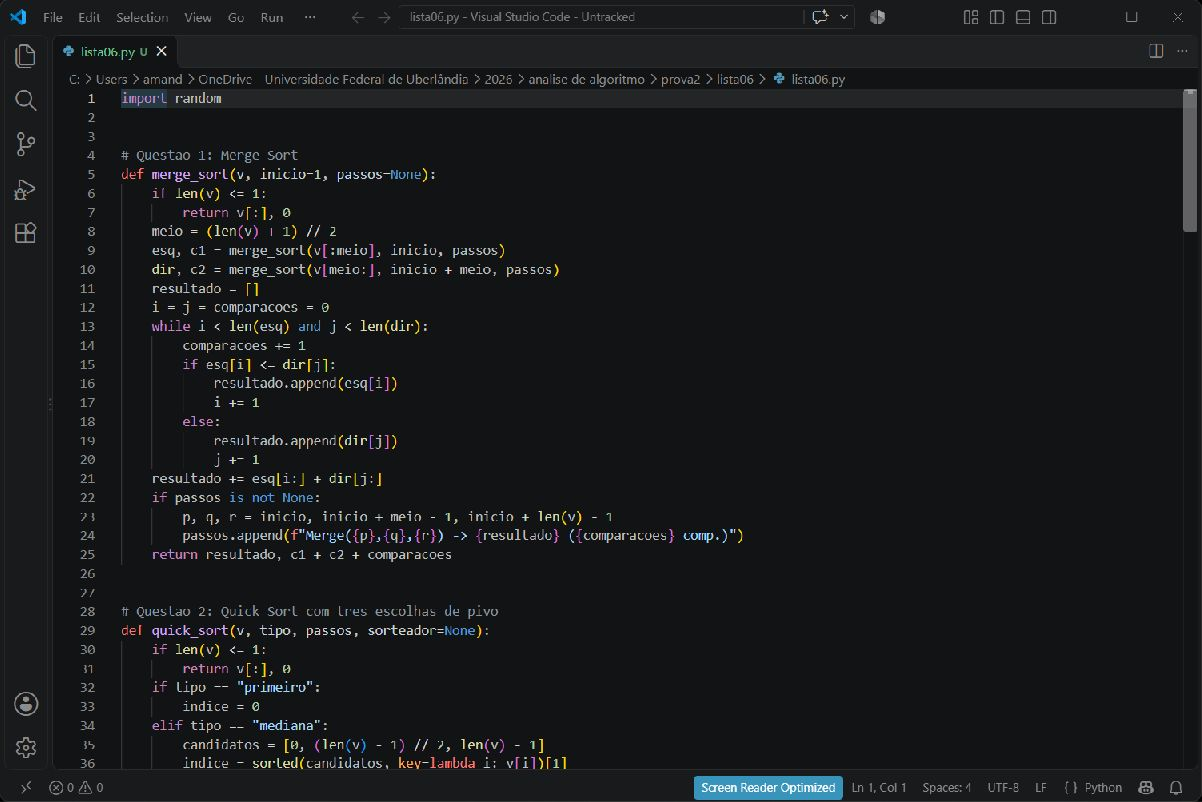
\includegraphics[width=15.6cm]{codigo_1.png}

\small Código aberto no VS Code.
\end{center}

\newpage
\section*{Questão 2 -- Quick Sort}
Testei as três escolhas de pivô no mesmo vetor. Com o primeiro elemento, as divisões ficam desequilibradas e ocorreram 45 comparações. Com a mediana de três, foram 19. A execução aleatória, usando uma semente fixa para repetir o teste, fez 28 comparações. Assim, o primeiro caso tem custo $O(n^2)$ nessa entrada; os outros têm custo esperado ou balanceado $O(n\log n)$.

\begin{center}
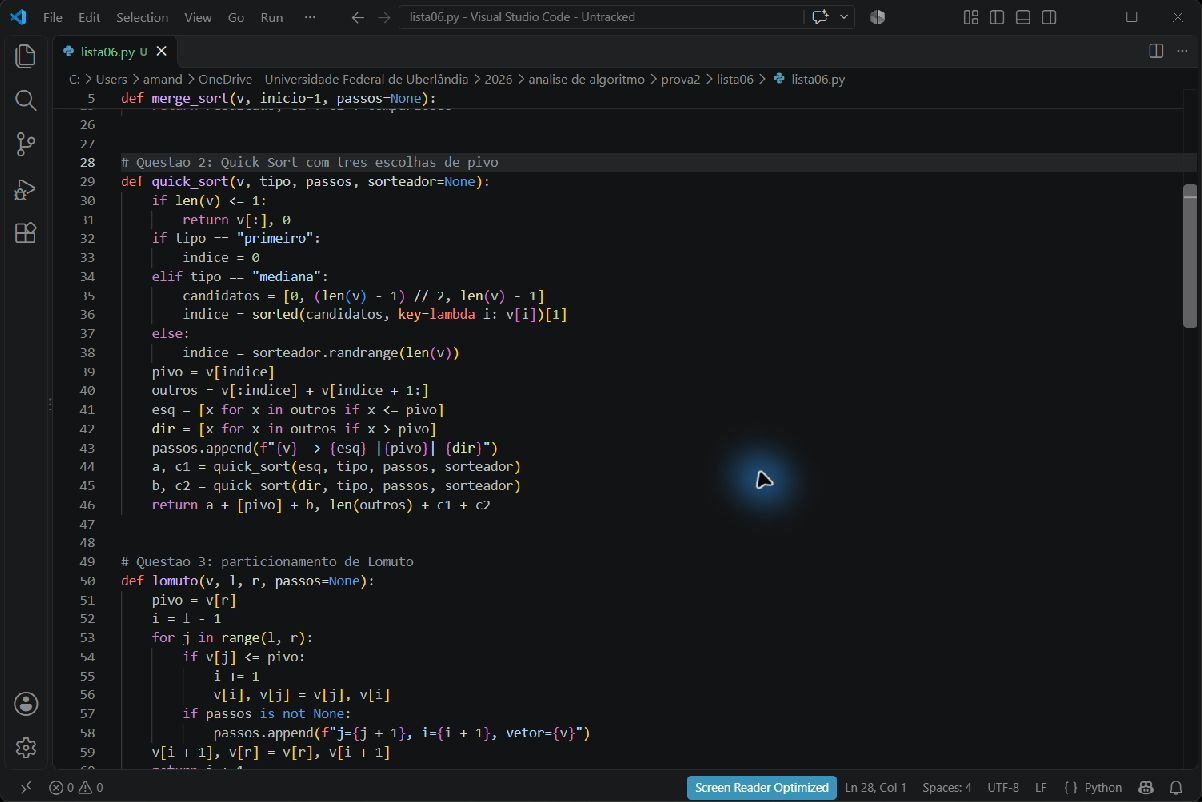
\includegraphics[width=15.6cm]{codigo_2.png}

\small Código das três escolhas de pivô.
\end{center}

\newpage
\section*{Questão 3 -- Partition-Lomuto}
O pivô é 10, o maior valor da entrada. Por isso, nas nove passagens do laço, cada elemento é trocado com ele mesmo; no fim, o pivô fica na posição 10. O invariante é: antes de cada passo, os valores até $i$ são menores ou iguais ao pivô, e os valores entre $i+1$ e $j-1$ são maiores. Cada comparação mantém essa separação. A troca final coloca o pivô entre os dois grupos, comprovando a correção. O laço percorre $n-1$ elementos: tempo $O(n)$ e espaço extra $O(1)$.

Coloquei um breakpoint dentro do laço para acompanhar a execução. No print, o depurador está parado antes da comparação, mostrando o pivô 10, os índices $i=-1$ e $j=0$, o vetor e a pilha de chamadas.

\begin{center}
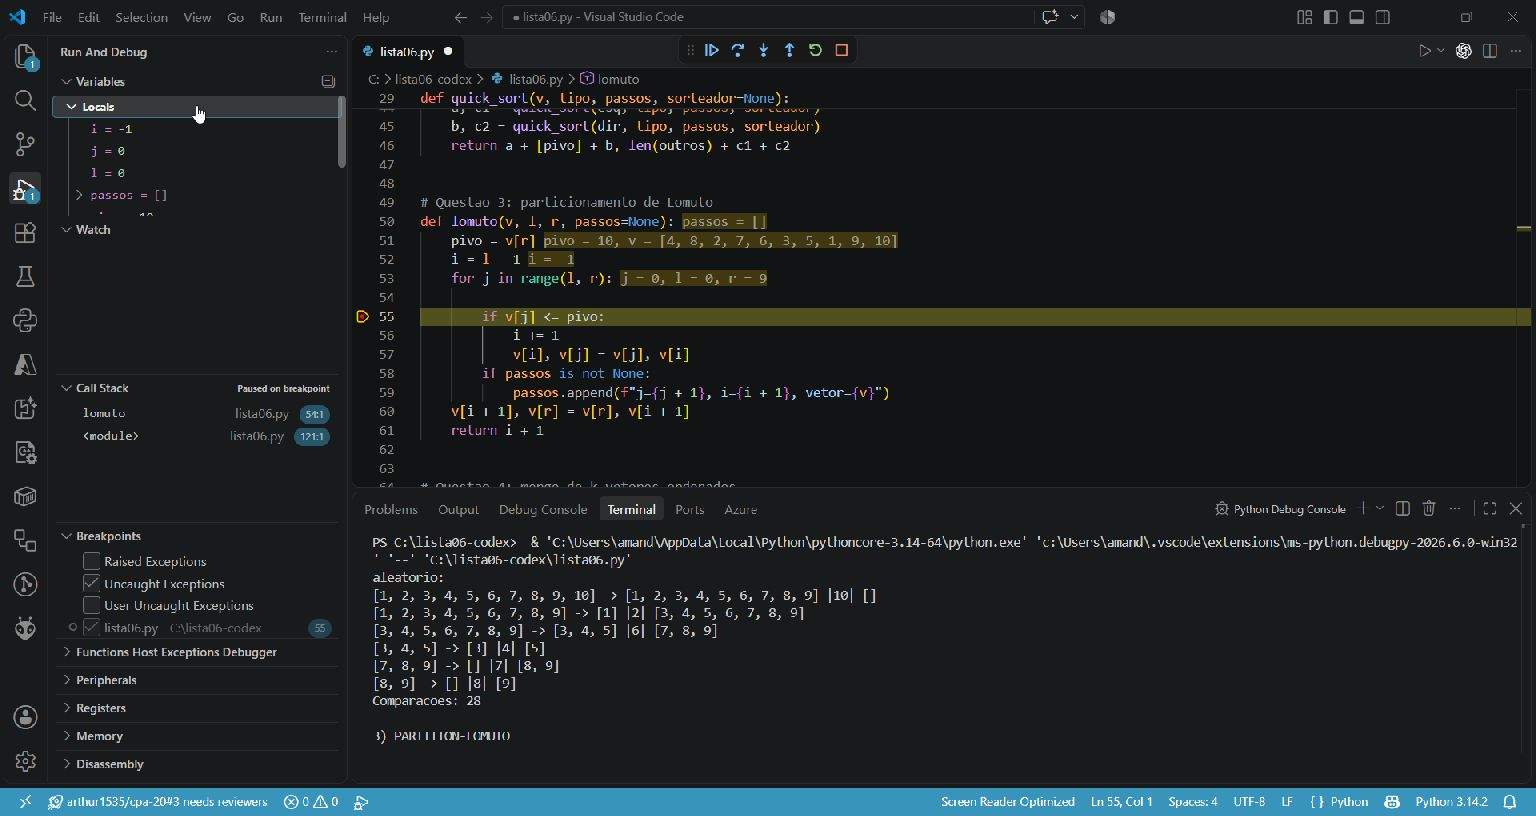
\includegraphics[width=15.6cm]{debug_exercicio3.png}

\small Exercício 3 rodando no depurador do VS Code.
\end{center}

\newpage
\section*{Questão 4 -- Merge de $k$ vetores}
Dividi os vetores em dois grupos, resolvi cada grupo e intercalei os resultados. Em cada nível são processados $nk$ elementos; como há $\log k$ níveis, o custo é $O(nk\log k)$. No exemplo, três vetores de três elementos formaram $[1,2,3,4,5,6,7,8,9]$.

\begin{center}
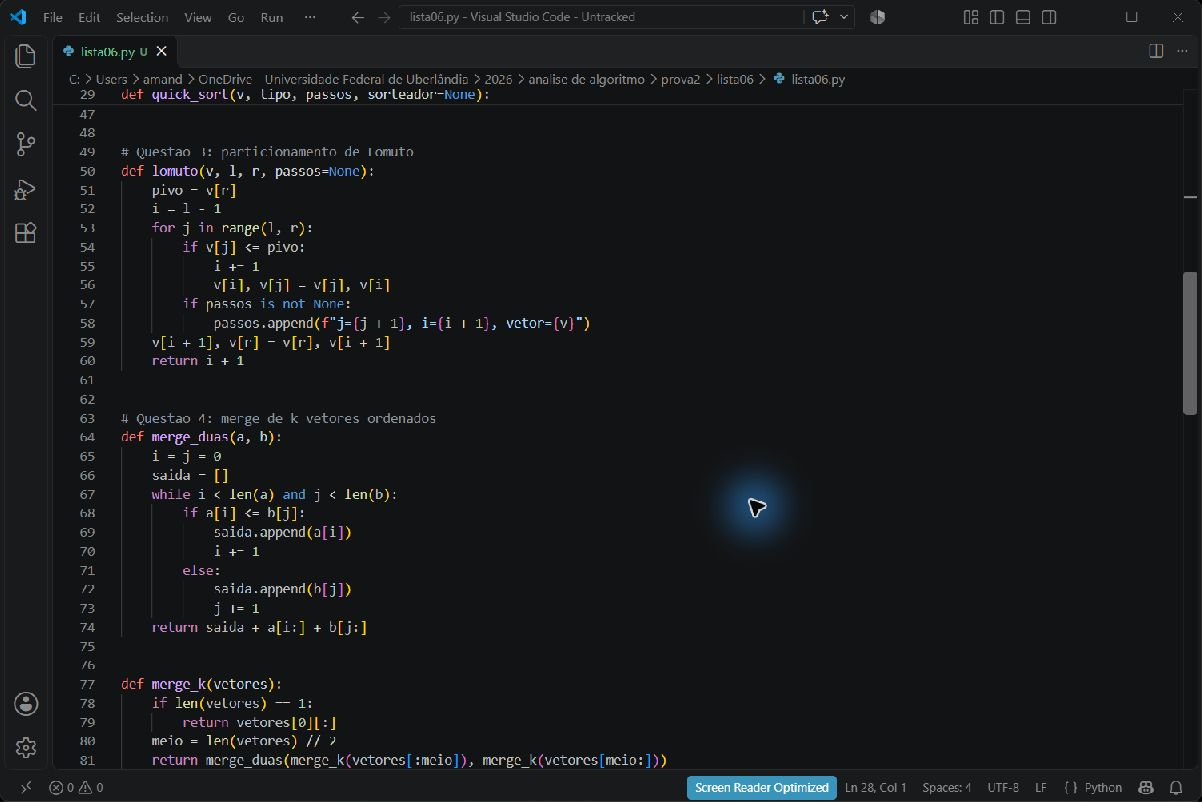
\includegraphics[width=12.8cm]{codigo_3.png}

\small Código do particionamento e da intercalação usado no programa.

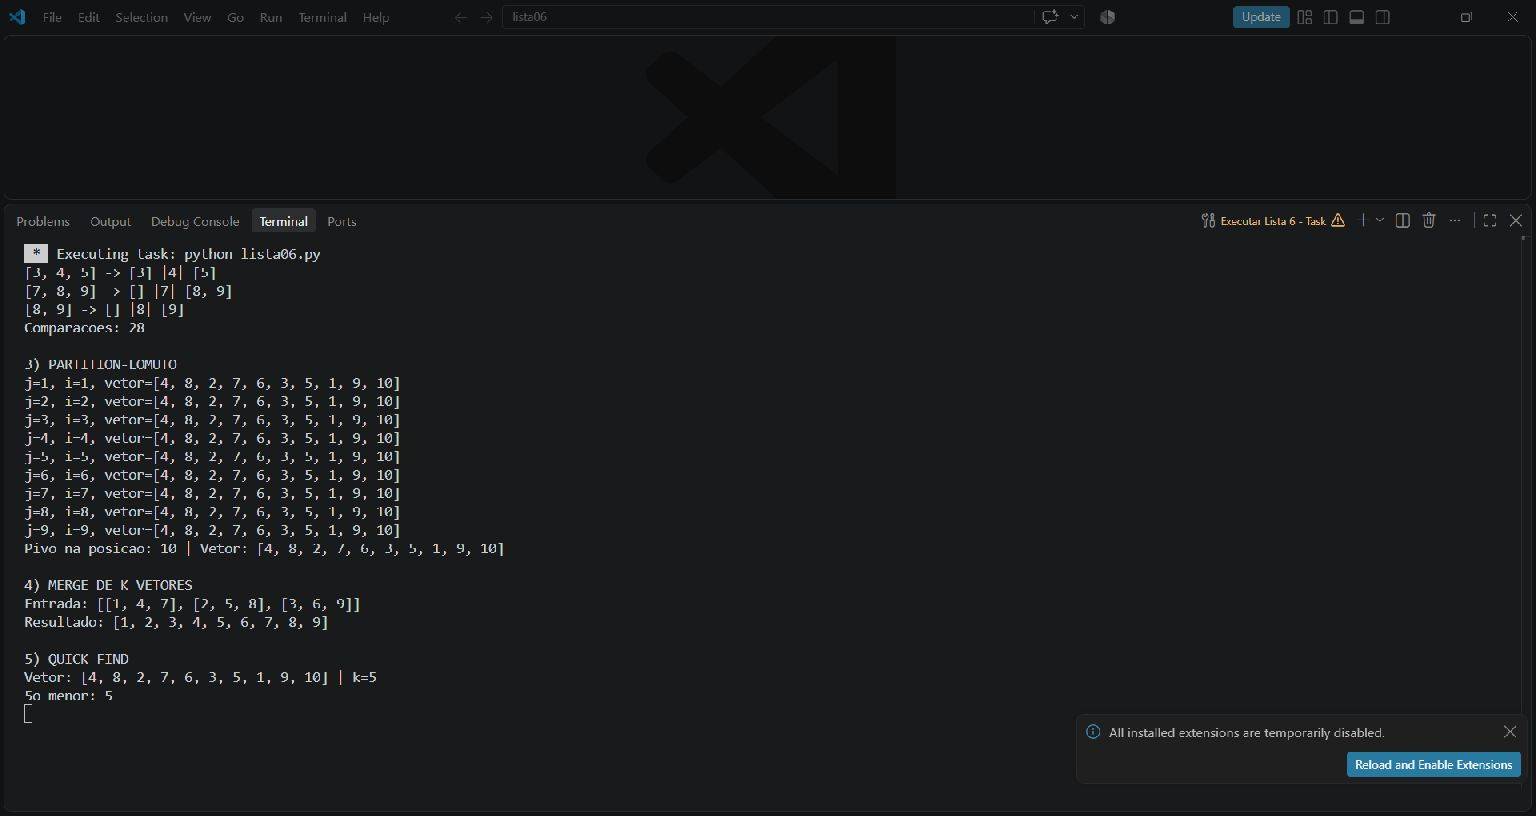
\includegraphics[width=13.8cm]{terminal_execucao.png}

\small Execução no terminal do VS Code. O comando \texttt{python lista06.py} aparece no início do terminal e o programa terminou mostrando os resultados.
\end{center}

\newpage
\section*{Questão 5 -- Quick-Find}
Usei o particionamento de Lomuto com pivô sorteado. Depois de cada partição, procurei somente no lado que pode conter o $k$-ésimo menor. Para $k=5$, o programa encontrou o valor 5, mostrado no print da página anterior.

O enunciado cita $O(\log n)$ no caso médio. Esse é o número típico de níveis percorridos, mas não o tempo total: cada partição percorre o trecho atual do vetor. O tempo esperado é $O(n)$ e o pior caso é $O(n^2)$.

\begin{center}
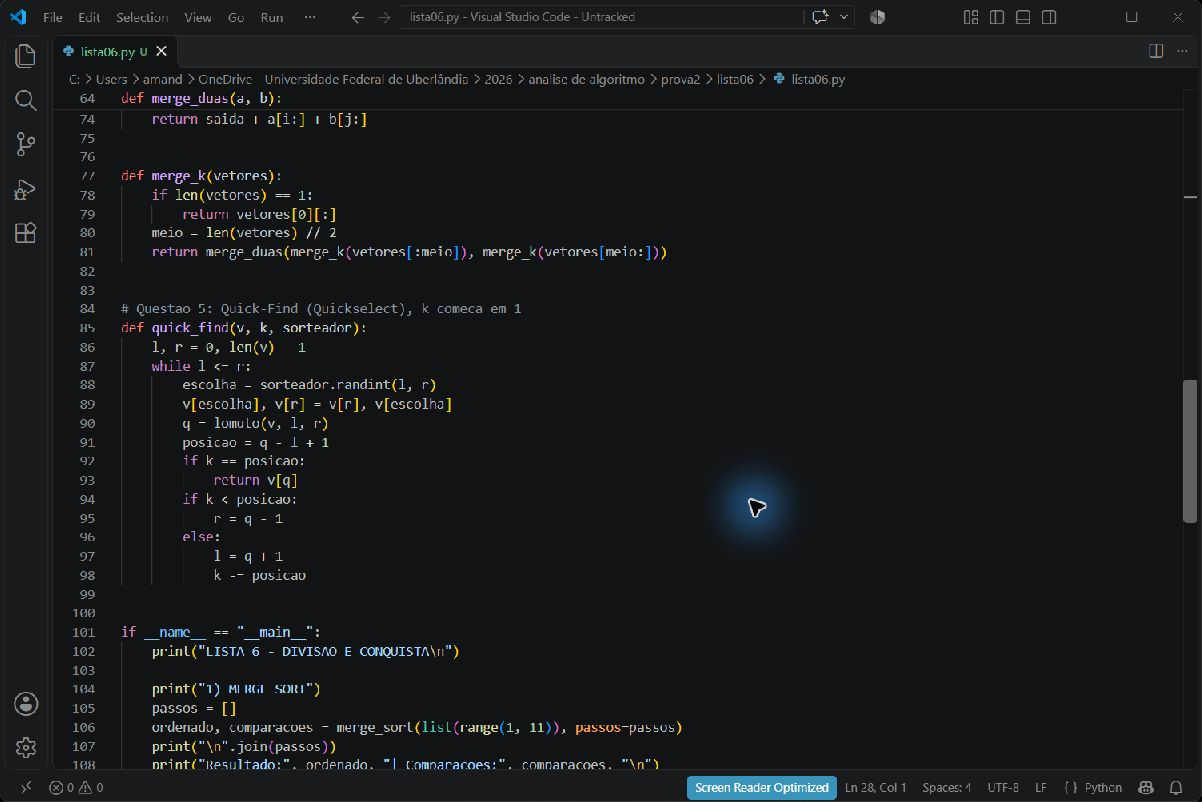
\includegraphics[width=15.6cm]{codigo_4.png}

\small Código do Quick-Find aberto no VS Code.
\end{center}

\end{document}
